\begin{definition}
Une {\em erreur de corr\'elation} est l'existence ou l'absence de corr\'elation entre deux ar\^etes (ou arcs) lorsque, respectivement, il n'existe pas de corr\'elations ou il en existe une.
\newline
L'absence de corr\'elation (corr\'elation {\em fausse n\'egative}) est d\'esign\'ee par $0$ dans la matrice d'adjacence tandis que l'existence de corr\'elation (corr\'elation {\em fausse positive}) a une valeur $1$ dans cette matrice. 
\end{definition}

\begin{definition}
Une corr\'elation entre ar\^etes (ou arcs) est l'existence d'un sommet commun aux ar\^etes (ou arcs). Ce sommet commun peut \^etre source, destination ou interm\'ediaire comme present\'e dans la figure \ref{typeSommetEnCommun}
\begin{centering} 
\begin{figure}[htb!] 
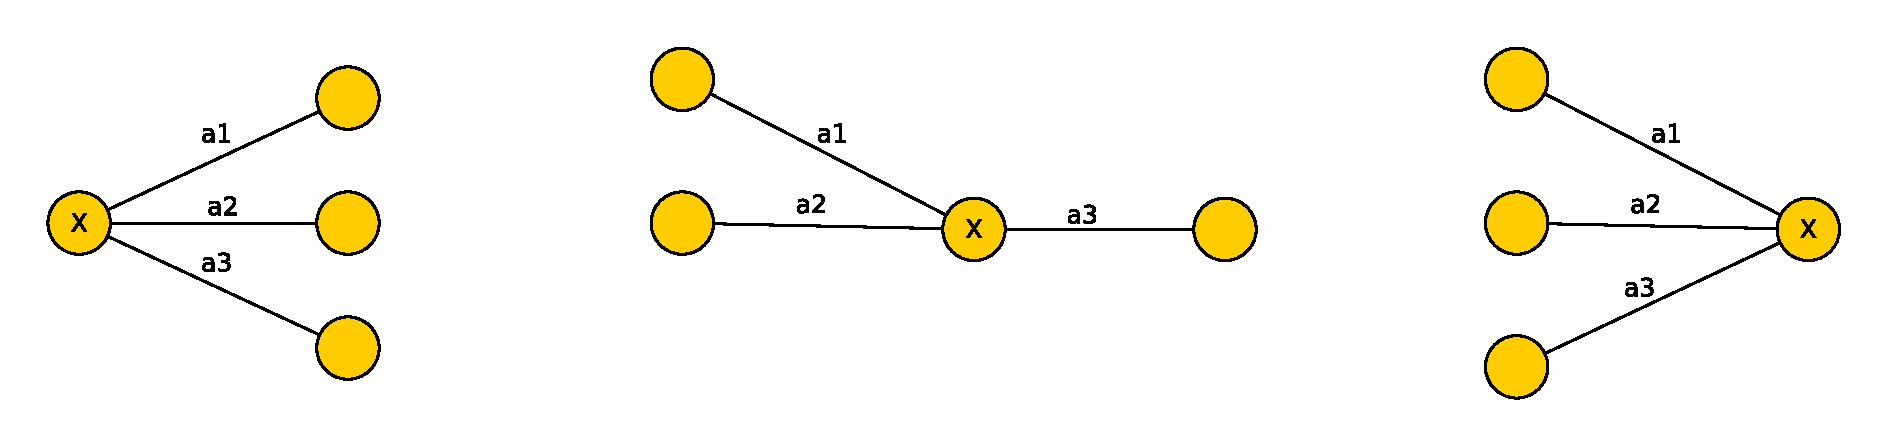
\includegraphics[scale=0.50]{images/typeSommetsEnCommun.eps}
\caption{De la gauche \`a la droite: sommet $X$ source, sommet $X$ interm\'ediaire, sommet $X$ destination}
\label{typeSommetEnCommun} 
\end{figure}
\end{centering} 
\end{definition}

\begin{definition}{ m\'etrique: distance de Hamming} \newline
La m\'etrique utilis\'ee pour diff\'erencier deux graphes est la {\em distance de Hamming}.
La distance de Hamming est le nombre d'ar\^etes (ou arcs) diff\'erentes entre deux graphes ayant le m\^eme ensemble de sommets. 
\end{definition}
Ainsi, une distance de Hamming \'egale \`a $0$ signifie que les deux graphes sont identiques. Tandis que  une distance de Hamming \'egale \`a $k$ signifie qu'il a $k$ ar\^etes diff\'erentes entre ces deux graphes.

\begin{definition}{ fonction de c\^out d'un sommet} \newline
La fonction de c\^out d'un sommet est le c\^out de chaque ar\^ete ajout\'ee ou supprim\'ee lorsqu'on applique l'algorithme de correction sur ce sommet.
\end{definition}
Le co\^ut d'une ar\^ete peut \^etre
\begin{itemize}
	\item unitaire : l'ajout et la suppression valent $1$.
	\item normal: la suppression est la probabilit\'e de l'ar\^ete et l'ajout vaut  $1$ moins cette probabilit\'e.
	\item carr\'e : la suppression est la probabilit\'e au carr\'e de l'ar\^ete et l'ajout vaut  $1$ moins cette probabilit\'e au carr\'e.
	\item quadratique :  la suppression est la probabilit\'e de l'ar\^ete \`a la puissance $4$ et l'ajout vaut  $1$ moins cette probabilit\'e \`a la puissance $4$.
\end{itemize}